\definecolor{Red}{RGB}{217,33,32}
\definecolor{Blue}{RGB}{63,96,174}
\definecolor{Duck}{RGB}{83,158,182}
\definecolor{Green}{RGB}{109,179,136}
\definecolor{Yellow}{RGB}{202,184,67}
\definecolor{Orange}{RGB}{231,133,50}
\definecolor{Purple}{RGB}{120,28,129}
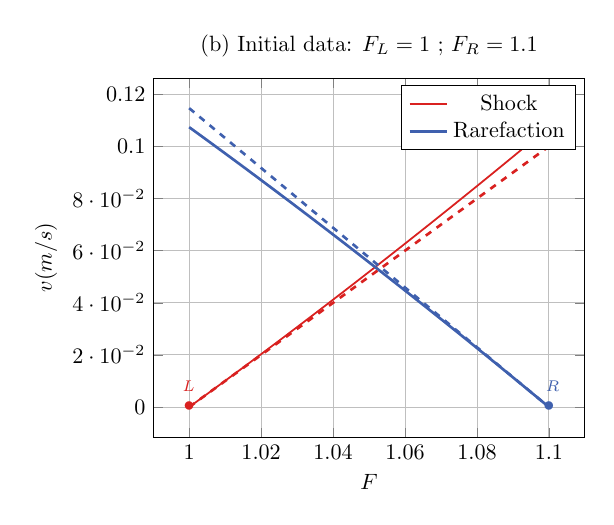
\begin{tikzpicture}[scale=0.8]
\begin{axis}[xlabel=$F$,ylabel=$v (m/s)$,ymajorgrids=true,xmajorgrids=true,title={(b) Initial data: $F_L=1$ ; $F_R=1.1$}]
\addplot[Red,thick] coordinates {(1.0,0.0) (1.001960196019602,0.0019630775609053948) (1.003920392039204,0.003931917267080632) (1.005880588058806,0.005906517718693416) (1.0078407840784078,0.007886877524091035) (1.00980098009801,0.009872995299740863) (1.0117611761176117,0.011864869670167599) (1.0137213721372138,0.01386249926789511) (1.0156815681568157,0.01586588273338493) (1.0176417641764177,0.01787501871497885) (1.0196019601960196,0.019889905868838792) (1.0215621562156216,0.02191054285889049) (1.0235223522352235,0.023936928356764118) (1.0254825482548255,0.025969061041739377) (1.0274427442744274,0.028006939600686957) (1.0294029402940295,0.030050562728014697) (1.0313631363136313,0.03209992912561001) (1.0333233323332334,0.034155037502787186) (1.0352835283528352,0.0362158865762309) (1.0372437243724373,0.03828247506994398) (1.0392039203920391,0.04035480171519238) (1.0411641164116412,0.04243286525045405) (1.0431243124312433,0.044516664421364406) (1.045084508450845,0.04660619798066565) (1.0470447044704472,0.048701464688155255) (1.049004900490049,0.050802463310633685) (1.050965096509651,0.05290919262185532) (1.052925292529253,0.055021651402476585) (1.054885488548855,0.05713983844000798) (1.0568456845684568,0.059263752528762766) (1.058805880588059,0.06139339246981025) (1.0607660766076608,0.06352875707092508) (1.0627262726272628,0.06566984514654145) (1.0646864686468647,0.06781665551770343) (1.0666466646664667,0.06996918701201955) (1.0686068606860686,0.07212743846361445) (1.0705670567056706,0.07429140871308419) (1.0725272527252725,0.07646109660744838) (1.0744874487448746,0.07863650100010654) (1.0764476447644764,0.08081762075079126) (1.0784078407840785,0.08300445472552491) (1.0803680368036805,0.08519700179657394) (1.0823282328232824,0.08739526084240548) (1.0842884288428845,0.08959923074764438) (1.0862486248624863,0.09180891040302837) (1.0882088208820884,0.09402429870536706) (1.0901690169016902,0.09624539455749745) (1.0921292129212923,0.09847219686824406) (1.0940894089408941,0.1007047045523746) (1.0960496049604962,0.10294291653056116) (1.098009800980098,0.1051868317293367) (1.0999699969997,0.10743644908105657) };
\addplot[Blue,very thick] coordinates {(1.0,0.1073874627707086) (1.001960196019602,0.10542438591418365) (1.003920392039204,0.10345555112494406) (1.005880588058806,0.10148096397787983) (1.0078407840784078,0.09950062999930058) (1.00980098009801,0.09751455466754301) (1.0117611761176117,0.09552274341357074) (1.0137213721372138,0.09352520162156171) (1.0156815681568157,0.0915219346294884) (1.0176417641764177,0.089512947729686) (1.0196019601960196,0.08749824616941433) (1.0215621562156216,0.08547783515140679) (1.0235223522352235,0.08345171983441528) (1.0254825482548255,0.08141990533374051) (1.0274427442744274,0.07938239672176006) (1.0294029402940295,0.07733919902844166) (1.0313631363136313,0.0752903172418546) (1.0333233323332334,0.07323575630866758) (1.0352835283528352,0.07117552113464229) (1.0372437243724373,0.06910961658511733) (1.0392039203920391,0.06703804748548585) (1.0411641164116412,0.06496081862166392) (1.0431243124312433,0.06287793474055453) (1.045084508450845,0.06078940055050131) (1.0470447044704472,0.05869522072173673) (1.049004900490049,0.056595399886824015) (1.050965096509651,0.05448994264109064) (1.052925292529253,0.05237885354305752) (1.054885488548855,0.05026213711485809) (1.0568456845684568,0.0481397978426566) (1.058805880588059,0.04601184017705303) (1.0607660766076608,0.04387826853348905) (1.0627262726272628,0.0417390872926421) (1.0646864686468647,0.0395943008008181) (1.0666466646664667,0.037443913370333926) (1.0686068606860686,0.03528792927989956) (1.0705670567056706,0.03312635277498877) (1.0725272527252725,0.03095918806820985) (1.0744874487448746,0.02878643933966615) (1.0764476447644764,0.026608110737315303) (1.0784078407840785,0.0244242063773199) (1.0803680368036805,0.022234730344396287) (1.0823282328232824,0.020039686692156212) (1.0842884288428845,0.017839079443443134) (1.0862486248624863,0.01563291259066641) (1.0882088208820884,0.013421190096127349) (1.0901690169016902,0.011203915892344065) (1.0921292129212923,0.008981093882367926) (1.0940894089408941,0.006752727940100287) (1.0960496049604962,0.00451882191059879) (1.098009800980098,0.0022793796103861676) (1.0999699969997,3.4404827748516585e-05) };
\node at (axis cs:1,0) [Red] {$\bullet$};
  \node at (axis cs:1.1,0) [Blue] {$\bullet$};
  \node at (axis cs:1,0) [anchor=south,Red] {$\Qcb^L$};
  \node at (axis cs:1.097,0) [above right,Blue] {$\Qcb^R$};
  \addplot[Red,dashed,very thick,domain=1:1.1,samples=51,samples y=0]
  ({x},{0.+sqrt(0.5*(3.-1))*(x-1.)});
  \addplot[Blue,dashed,very thick,domain=1:1.1,samples=51,samples y=0]
    ({x},{0.-sqrt(0.5*(3.*(1.1^2)-1))*(x-1.1)});
\legend{Shock,Rarefaction}
\end{axis}
\end{tikzpicture}
